\documentclass[10pt]{beamer}

\usetheme[progressbar=frametitle]{metropolis}
\usepackage{appendixnumberbeamer}

\usepackage{booktabs}
\usepackage[scale=2]{ccicons}

\usepackage{pgfplots}
\usepgfplotslibrary{dateplot}

\usepackage{xspace}
\newcommand{\themename}{\textbf{\textsc{metropolis}}\xspace}

\usepackage{array}
\usepackage{longtable}
\usepackage{rotating}
\usepackage{float}
\usepackage{rotfloat}
\usepackage{multirow}
\usepackage{amssymb}
\usepackage{graphicx}
\usepackage{setspace}
\usepackage{nomencl}


%Packages of mindmap

\usepackage[utf8]{inputenc}
%\usepackage{dtklogos}
\usepackage{tikz}
\usetikzlibrary{mindmap,shadows}
% Information boxes
\newcommand*{\info}[4][16.3]{%
  \node [ annotation, #3, scale=0.65, text width = #1em,
          inner sep = 2mm ] at (#2) {%
  \list{$\bullet$}{\topsep=0pt\itemsep=0pt\parsep=0pt
    \parskip=0pt\labelwidth=8pt\leftmargin=8pt
    \itemindent=0pt\labelsep=2pt}%
    #4
  \endlist
  };
}

% Tikz

\definecolor{myblue}{HTML}{020364}
\usetikzlibrary{shapes,arrows,matrix,decorations.pathreplacing,shapes.geometric,positioning}  
% Gantt
\usepackage{pgfgantt}
\usepackage{adjustbox} %Ajustar a la página


\title{Passive dynamic system for energy returning on trans-tibial prosthesis}
\subtitle{Reformed Objectives and Schedule}
\date{\today}
\date{}
\author{Nikolay Prieto M.Sc.}
\institute{Universidad Nacional de Colombia}
\titlegraphic{\hfill
\includegraphics[height=1.5cm]{2.png}}

\begin{document}

\maketitle

\begin{frame}{Table of contents}
  \setbeamertemplate{section in toc}[sections numbered]
  \tableofcontents[hideallsubsections]
\end{frame}

\section{Introduction}

\begin{frame}[fragile]{Introduction}

The purpose of this presentation is to let you know the general activities done to date, and to propose the reformed objectives and activities for this year.

\end{frame}
\begin{frame}[fragile]{Background of the objectives}

\begin{alertblock}{General Objective} 
To suggest an ankle-foot prosthesis being able to generate --- through a passive dynamic system --- the positive work needed for push-off after dual-flexion phase, taking advantage of the energy lost at initial contact of the gait.
\end{alertblock}

\end{frame}

\begin{frame}[fragile]{Background of the objectives}

\begin{alertblock}{Specific Objectives}
\begin{enumerate}

\item Identify biomechanical parameters and the work-loop slope of ESR prosthesis users and non-amputees aiming to obtain the ankle quasi-stiffness of both cases.

\item Obtain a preliminary model of the ankle-foot prosthesis capable of storing energy (during initial contact until late dual-flexion phase), and returning it at dorsi-flexion phase in a controlled manner through the passive dynamic system.

\item Determine detailed configurations of cellular solids that accomplish the requirements of the preliminary model.
\item Validate the dynamic model of the ankle-foot prosthesis in comparison to an ESR prosthesis. \end{enumerate}

\end{alertblock}
\end{frame}

\begin{frame}{Schedule proposed}

\begin{ganttchart}[
x unit=0.2cm,
y unit title=0.5cm,
y unit chart=0.3cm,
vgrid,
time slot format=isodate-yearmonth,
compress calendar,
title/.append style={draw=none, fill=myblue},
title label font=\footnotesize\sffamily\bfseries\color{white},
title label node/.append style={below=-1.6ex},
title left shift=.05,
title right shift=-.05,
title height=0.5,
bar/.append style={draw=none, fill=green!75},
bar height=.3,
bar label font=\normalsize\color{black!50},
group right shift=0,
group top shift=.6,
group height=.3,
group peaks height=.2,
bar incomplete/.append style={fill=brown}
]{2016-04}{2018-12}
\gantttitlecalendar{year} \\
\ganttbar[
progress=100,
bar progress label font=\small\color{black},
bar progress label node/.append style={right=4pt},
bar label font=\footnotesize\color{black!50},
name=pp
]{{\scriptsize Doctoral Proposal}}{2016-04}{2016-06} \\
\ganttset{progress label text={}, link/.style={black, -to}}
\ganttgroup{{\footnotesize Objective 1}}{2016-06}{2017-03}\\ 
\ganttbar[progress=100, name=T1A]{{\scriptsize Obtaining data from the literature}}{2016-06}{2016-07} \\
\ganttbar[progress=100, name=T1A]{\scriptsize Filtering data}{2016-07}{2016-08} \\
\ganttbar[progress=100, name=T1A]{\scriptsize Obtaining biomechanical model}{2016-08}{2016-10} \\
\ganttbar[progress=100, name=T1A]{\scriptsize Getting ankle quasi-stiffness}{2016-10}{2016-12} \\
\ganttbar[progress=100, name=T1A]{\scriptsize Verificating results}{2017-01}{2017-03} \\
\ganttgroup{\footnotesize Objective 2}{2017-06}{2017-12} \\
\ganttbar[progress=0, name=T2A]{\scriptsize Including loads and constrains}{2017-06}{2017-08} \\
\ganttbar[progress=0, name=T2A]{\scriptsize Determining geometries}{2017-08}{2017-10} \\
\ganttbar[progress=0, name=T2A]{\scriptsize Optimizing sub-domains}{2017-10}{2017-07} \\
\ganttbar[progress=0, name=T2A]{\scriptsize Obtaining preliminary design}{2017-07}{2017-10} \\
\ganttbar[progress=0, name=T2A]{\scriptsize Simulate preliminary design}{2017-08}{2017-12} \\
\ganttgroup{\footnotesize Objective 3}{2017-10}{2018-06} \\
\ganttbar[progress=0]{\scriptsize Cellular solids configurations}{2017-10}{2018-01}\\
\ganttbar[progress=0, name=T2A]{\scriptsize Verifying energetic storage}{2017-12}{2018-04} \\
\ganttbar[progress=0, name=T2A]{\scriptsize Optimizing design}{2017-12}{2018-04} \\
\ganttbar[progress=0, name=T2A]{\scriptsize Obtaining quasi-stiffness from model}{2018-04}{2018-06} \\
\ganttgroup{\footnotesize Objective 4}{2018-06}{2018-12} \\
\ganttbar[progress=0]{\scriptsize Manufacturing process}{2018-06}{2018-08}\\
\ganttbar[progress=0, name=T2A]{\scriptsize Ethical procedures and testing}{2018-08}{2018-10} \\
\ganttbar[progress=0, name=T2A]{\scriptsize Validating prototype model}{2018-10}{2018-12} \\
\ganttgroup{\scriptsize Writing thesis and papers}{2016-10}{2018-12} \\
\ganttset{link/.style={black}}
%\ganttlink[link mid=.4]{pp}{T1A}
%\ganttlink[link mid=.159]{pp}{T2A}
\end{ganttchart}
\end{frame}

\section{Modifications}

\begin{frame}{Purpose No. 01}
	\begin{block}{Option A}
	Through the extraction of experimental data, we will identify the biomechanical parameters and the work-loop slope in ESR prosthesis users and non-amputees, aiming to obtain the ankle quasi-stiffness of both cases.
	\end{block}
	\begin{exampleblock}{Deliverables}
	An article relating the Dynamic Joint Stiffness of the ankle-joint --- and other joints if it is possible --- of a good statistical sample of lower limb amputees.
	\end{exampleblock}
\end{frame}

\begin{frame}{Activities and Schedule}
\begin{ganttchart}[
x unit=0.8cm,
y unit title=0.7cm,
y unit chart=0.8cm,
vgrid,
time slot format=isodate-yearmonth,
compress calendar,
title/.append style={draw=none, fill=myblue},
title label font=\footnotesize\sffamily\bfseries\color{white},
title label node/.append style={below=-1.6ex},
title left shift=.05,
title right shift=-.05,
title height=1,
bar/.append style={draw=none, fill=green!75},
bar height=.6,
bar label font=\normalsize\color{black!50},
group right shift=0,
group top shift=.6,
group height=.3,
group peaks height=.2,
bar incomplete/.append style={fill=brown},
vgrid={*{2}{dotted},{green,ultra thick},*{11}{dotted}}
]{2018-01}{2018-06}
\gantttitlecalendar{year} \\
\ganttset{progress label text={}, link/.style={black, -to}}
\ganttgroup{Ph.D Thesis}{2018-01}{2018-06}\\ 
\ganttbar[progress=100, name=T1A]{Filtering the most useful data}{2018-01}{2018-01} \\
\ganttbar[progress=0, name=T1A]{Ethical committee}{2018-01}{2018-02} \\
\ganttbar[progress=0, name=T1A]{Selecting the appropriate population}{2018-01}{2018-03} \\
\ganttbar[progress=0, name=T1A]{Obtaining biomechanical model}{2018-02}{2018-04} \\
\ganttbar[progress=0, name=T1A]{Getting ankle quasi-stiffness}{2018-03}{2018-05} \\
\ganttbar[progress=0, name=T1A]{Obtain energetic loss at collision}{2018-05}{2018-06} \\

\end{ganttchart}
\end{frame}

\begin{frame}{Purpose No. 01}
	\begin{block}{Option B}
	Through the analysis of pure data found in the literature, we will attempt to give insights about the dynamic behaviour of the ankle could describe unseen aspects of different types of gait and also to identify non-linear approximations of the quasi-stiffness. 
	\end{block}
	\begin{exampleblock}{Deliverables}
	An article relating a methodology to give more accuracy in the linear regressions or predicting relationships between different parameters of the gait (i.e. Velocity, Body length, Body mass).
	\end{exampleblock}
\end{frame}

\begin{frame}{Example of analyzed data}
\begin{figure}[H]
\begin{centering}
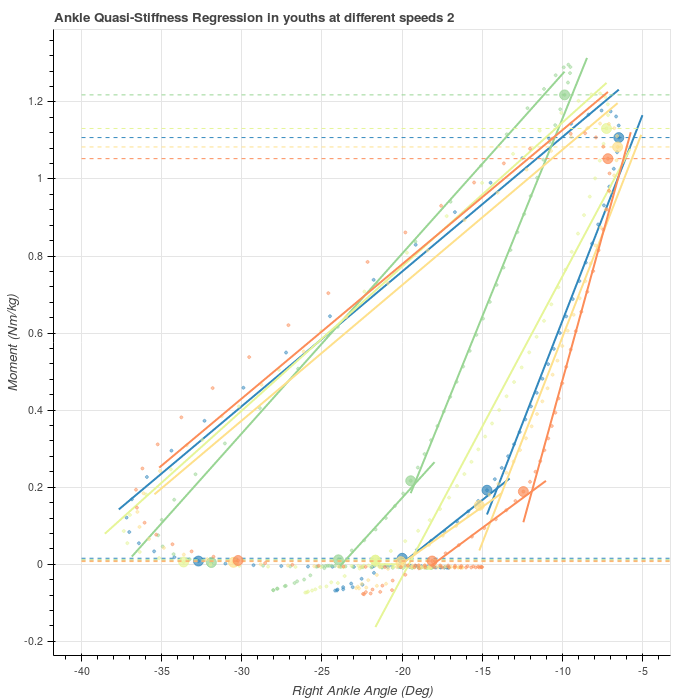
\includegraphics[scale=0.25]{quasistiffness.png}
\par\end{centering}

\caption{\label{fig:N=1} Dynamic Joint Stiffness of the ankle, being linearized according to each sub-phase of the gait}

\end{figure}
\end{frame}

\begin{frame}{Purpose No. 02}
	\begin{block}{Option B}
	Trying to get a topology optimization algorithm for the optimal design of cellular materials and composites with periodic microstructures so that the resulting macro-structure has the maximum energy returning capacity. 
	\end{block}
	\begin{exampleblock}{Deliverables}
	Two articles, the first is with respect to the optimization algorithm, and the second one is related with the verification of the dynamical process of the gait.
	\end{exampleblock}
\end{frame}

\begin{frame}{Example of the optimization activity}
\begin{figure}[H]
\begin{centering}
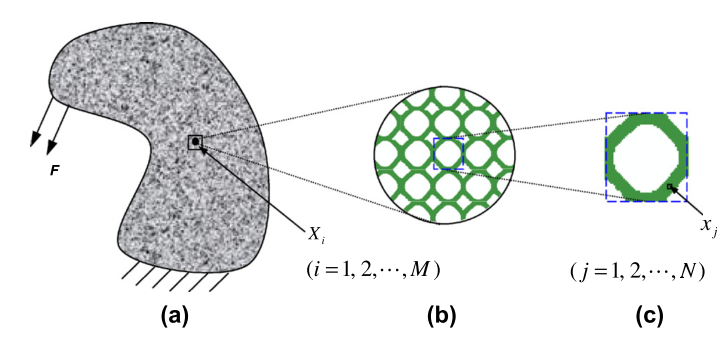
\includegraphics[scale=0.35]{optimiTopo.png}
\par\end{centering}

\caption{\label{fig:N=2} A structure composed of cellular materials or composites (a) macro-structure; (b) micro-structure; (c) a unit cell.}

\end{figure}
\end{frame}

\begin{frame}{Internship}
\begin{ganttchart}[
x unit=0.6cm,
y unit title=0.7cm,
y unit chart=0.8cm,
vgrid,
time slot format=isodate-yearmonth,
compress calendar,
title/.append style={draw=none, fill=myblue},
title label font=\footnotesize\sffamily\bfseries\color{white},
title label node/.append style={below=-1.6ex},
title left shift=.05,
title right shift=-.05,
title height=1,
bar/.append style={draw=none, fill=green!75},
bar height=.6,
bar label font=\normalsize\color{black!50},
group right shift=0,
group top shift=.6,
group height=.3,
group peaks height=.2,
bar incomplete/.append style={fill=brown},
]{2018-05}{2018-12}
%\gantttitlecalendar{year}{months} \\
\gantttitle[]{2018}{8} \\                 % title 
    \gantttitle{May}{1}
    \gantttitle{Jun}{1}
    \gantttitle{Jul}{1}
    \gantttitle{Aug}{1}
    \gantttitle{Sep}{1}
    \gantttitle{Oct}{1}
    \gantttitle{Nov}{1}
    \gantttitle{Dic}{1}\\
\ganttset{progress label text={}, link/.style={black, -to}}
\ganttgroup{Internship at IUPUI}{2018-06}{2018-12}\\ 
\ganttbar[progress=10, name=T1A]{{\footnotesize Developing computer algorithms}.}{2018-06}{2018-08} \\
\ganttbar[progress=0, name=T1A]{\footnotesize Tailoring cellular material configurations.}{2018-07}{2018-10} \\
\ganttbar[progress=0, name=T1A]{\footnotesize Physically testing cellular material configurations.}{2018-09}{2018-12} \\
\ganttbar[progress=0, name=T1A]{\footnotesize Attending lectures on Design Optimization.}{2018-06}{2018-12} \\
\ganttbar[progress=0, name=T1A]{\footnotesize Preparing one journal paper.}{2018-06}{2018-12} \\
\ganttset{link/.style={black}}
%\ganttlink[link mid=.4]{pp}{T1A}
%\ganttlink[link mid=.159]{pp}{T2A}
\end{ganttchart}

\end{frame}

\section{Questions}

\begin{frame}[standout]
  Thank you!
\end{frame}

\end{document}